% !TEX root = ../beamer.tex

\begin{frame}
    \frametitle{Modeling, Generation \& Deployment}
    
    \begin{center}   
	    \begin{tikzpicture}[
	    >=stealth,
	    every node/.style={outer sep = 0},
	    node distance = 0.75cm and 0.25cm,
	    big/.style = {draw, minimum width = 2.5cm, minimum height = 1.75em},
	    header/.style = {big, minimum width = 3.2cm, fill=pantone315!10!white, outer sep = 0}
	    ]
	    \node[header] (eclipseDevelopment) {Framework IDE\vphantom{Aq}};
	    \node[big, below = 0.2cm of eclipseDevelopment] (dsl) {DSL\vphantom{Aq}};
	    \node[big, below = 0.1cm of dsl] (generator) {Generator\vphantom{Aq}};
	    
	    \node[below=1.2cm of generator, header] (generatedArtifacts) {Generated Artifacts\vphantom{Aq}};
	    \node[big, below = 0.2cm of generatedArtifacts] (backend) {Backend\vphantom{Aq}};
	    \node[big, below = 0.1cm of backend] (mapApps) {\mapapps\vphantom{Aq}};
	    
	    \node[header, right = 2.3cm of backend, fill=pantone315!10!white] (glassfish) {Glassfish AS\vphantom{Aq}};
	    \node[header, right = 2.3cm of mapApps, fill=pantone315!10!white] (jetty) {Jetty};
	    
	    \draw[->] (backend) -- node[above] {\tiny{deploy}} (glassfish);
	    \draw[->] (mapApps) -- node[above] {\tiny{deploy}} (jetty);
	    
	    \node[header, right = 2cm of eclipseDevelopment] (eclipseModeling) {Modeling IDE\vphantom{Aq}};
	    \node[big, below = 0.2cm of eclipseModeling] (md2model) {\MD Model\vphantom{Aq}};
	    \node[big, below = 0cm of md2model, align=center] (modelModels) {models\\views\\controllers\\workflows};
	    
	    \draw[->] (md2model) -- node[above] {\tiny{uses}} (dsl);
	    \draw[->] (generator) -- node[left] {\tiny{generates}} (generatedArtifacts);
	    \draw[->] ($(eclipseModeling.south west) + (0, -1.3)$) -- node[above] {\tiny{invokes}} (generator);   

	    \draw (eclipseDevelopment.north west) rectangle ($(eclipseDevelopment.south east) + (0, -1.85)$);
	    \draw (generatedArtifacts.north west) rectangle ($(generatedArtifacts.south east) + (0, -1.85)$);
	    \draw (eclipseModeling.north west) rectangle ($(eclipseModeling.south east) + (0, -3.05)$);
	   % \draw (md2model.south west) rectangle ($(md2model.south east) + (0, -2.5)$);
	    
	    
	    \end{tikzpicture}
    \end{center}
\end{frame}

%-------------------------------------------------------------------------

\begin{frame}[fragile, plain]
	\plainnumber
    \frametitle{Use Case: Dating App}
    
    \begin{figure}
    	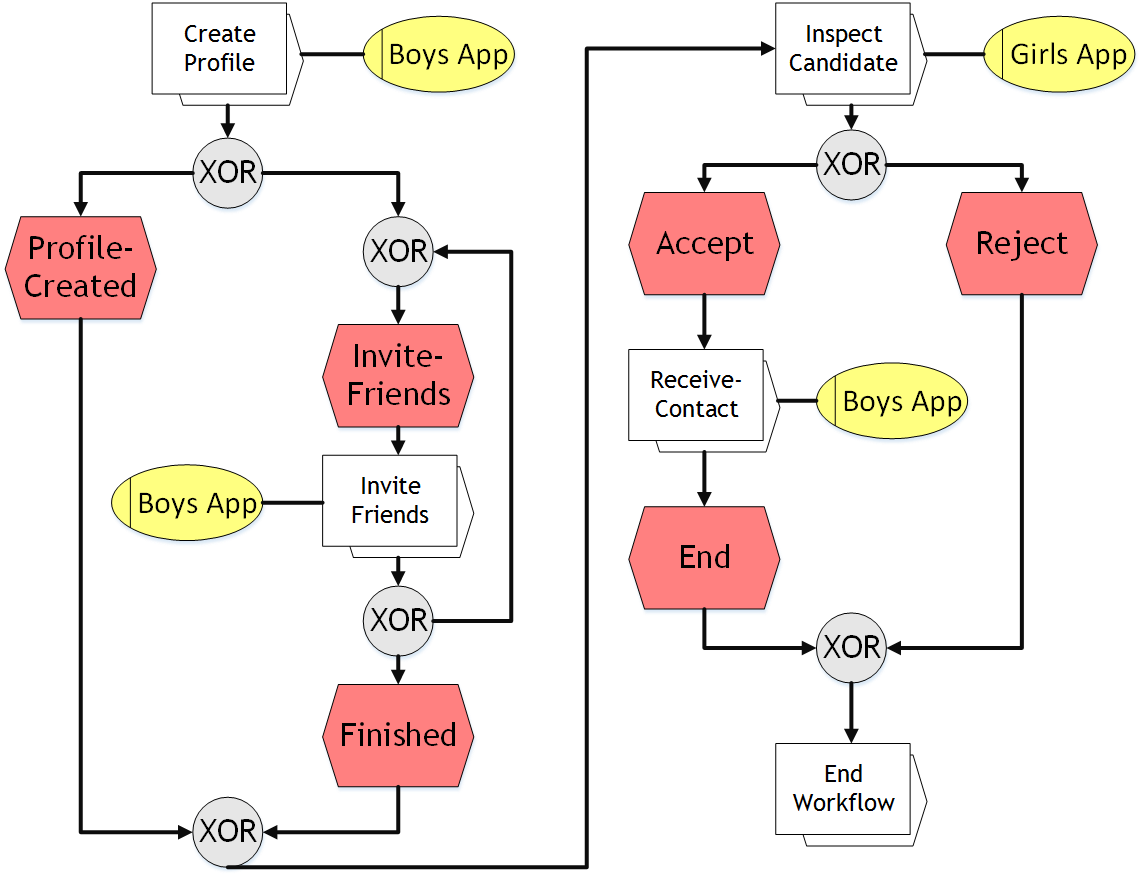
\includegraphics[width= 0.9\linewidth]{images/DatingApp.png}
    \end{figure}
\end{frame}
